\definecolor{grey}{HTML}{CCA3A3}
%couleur pour API REST

\begin{figure}[H]
\center

\includegraphics[width=0.2\textwidth]{elasticsearch.png}
\label{fig:elasticsearchlogo.png}
\end{figure}
\section{Introduction}
%Elasticsearch est notre backend, la colonne vertebrale de notre installation.
%C'est lui qui est capable d'analyser la masse de donnée

\section{Présentation de Elasticsearch}
Elasticsearch est moteur de recherche et d'analyse en temps réel. Il permet l'exploration
de données de façon très rapide par des recherches, que ce soit par des recherches
\gls{fulltext}, ou bien des recherches structurées.

Elasticsearch est depuis peu développé par la société \emph{Elastic}. C'était, à 
la base, un projet du développeur Shay Banon, qui souhaitait concevoir une API simplifié
pour la bibliothèque de moteur de recherche : Apache Lucene\fnu[Page du projet Lucene ]{https://lucenenet.apache.org/}.

Elasticsearch et la stack ELK est en passe de devenir un standard dans l'industrie.
En effet le logiciel à une utilisation assez versatile, de l'aide à la prise de 
décision en temps réelle à l'analyse de code source. Et à l'heure actuelle, la capacité 
à exploiter les masses de données et de méta données accumulées chaque jour devient 
un enjeu économique majeur. Enfin l'un des principaux 
atouts d'Elasticsearch réside dans son aptitude à pouvoir passer à l'échelle simplement.

\footnotesize{\emph{Attention, ce chapitre ne sera qu'une présentation très succinte des possibilités 
du logiciel Elasticsearch, tout détailler nécessiterait \emph{sans doutes} des milliers
de pages, le résumé officiel\footnote{Elasticsearch : The Definitive Guide, disponible 
chez Pearson et Github}
en fait déjà \emph{plus de 950} \ldots}}

\section{Installation}
Avant même de regarder les différentes dépendances nécessaires à l'utilisation de
Elasticsearch il est recommandé de vérifier que l'on utilise bien la même version
que son compère Logstash (vérifier la compatibilité dans la documentation si les
versions de Logstash et Elasticsearch ont un numéro différent).

Son installation est sensiblement la même que son comparse logstash puisque ce logiciel 
nécessite également l'installation des dépendances \emph{jruby} et \emph{openjdk-7-jre}
à noter qu'il fonctionne également sur openjdk-8-jre.

Là aussi les paquets debian officiels n'existant pas on utilisera celui fourni par 
\hyperref[https://download.elastic.co/elasticsearch/elasticsearch/elasticsearch-1.5.1.deb]{elastic.co}.

\subsection{Configuration de base}
Attention le paquet deb fourni (version 1.5) est loin d'être parfait.
Une fois l'installation achevé, il faudra rajouté un dossier config
dans \ipath{/usr/share/elasticsearch} et lui donner les droits qui conviennent.
\begin{lstlisting}[style=code,label={lst:ajoutdepotconfigchown}]
chown elasticsearch:elasticsearch
\end{lstlisting}

Enfin pour qu'Elasticsearch se lance, il faut au préalable renseigner le cluster.name
et le node.name dans \ipath{/etc/elasticsearch/elasticsearch.yml}.

Pour information tous les indices sont, par défaut, physiquement entreposé dans\\
\ipath{/usr/share/elasticsearch/data/}.



%p24-26
% test



\section{La théorie}
{%\huge A compléter}

%\subsection{Approximation et comparaison avec le modèle relationnel}
La comparaison entre Elasticsearch et un SGBD (système de gestion de base de données) 
n'est pas forcement heureuse, c'est un moteur de recherche (d'indexation), pas une 
base de données. 
%Il utilise donc la notion d'index qu'on peut cependant assez facilement comparer au modèle relationnel.

Cependant Elasticsearch s'organise autour d'index que l'on peut comparer aux bases (de données)
dans le modèle relationnel, un index peut utiliser plusieurs types\footnote{Dans 
notre projet \textbf{nous n'avons pas fait ce choix} pour pouvoir plus facilement 
modifier les mappings sans supprimer toutes les données. Il aurait été envisageable
par exemple de différencier les logs firewall des logs \textit{states} en utilisant 
les types. Cf partie 3}, ils s'apparentent aux tables dans le modèle relationnel. 

Chaque enregistrement d'Elasticsearch est effectué sous forme document. Les documents
sont nécessairement rangé dans un type, éventuellement type par défaut. Le document 
peut être comparé à une ligne (row). 

Ces lignes sont constituées de colonnes, appellées champs (ou fields) dans Elasticsearch.

\begin{figure}[H]
\textbf{BDD Relationnelle $\Rightarrow$ Base de données $\Rightarrow$ Tables $\Rightarrow$ Ligne $\Rightarrow$ Colonnes\\
Elasticsearch \hspace{7mm} $\Rightarrow$ \hspace{8mm }Index \hspace{8mm} $\Rightarrow$ \hspace{3mm}Types \hspace{3mm} $\Rightarrow$ Documents $\Rightarrow$ Champs}
\end{figure}


\section{L'infrastructure}
Dans cette partie nous allons expliquer comment fonctionne Elasticsearch à plus bas 
niveau. Nous allons parler de noeuds, de shards, d'instances\ldots

Comprendre cette partie est nécessaire pour pouvoir paramétrer une installation simple.
Nous expliquerons également les enjeux pour un cluster plus imposant.
\subsection{La base}
\label{subsec:labase}
\subsubsection{Grappes et nœuds}
Chaque instance d'Elasticsearch fonctionne nécessairement dans une entité abstraite 
appelé cluster (grappe), c'est son groupe. On peut avoir un cluster d'une seule instance.
Les clusters son identifiés par des noms.

Une instance est appelé \emph{node} (nœuds). Il est possible de lancer plusieurs nodes  
par machines mais c'est déconseillé (cf partie tuning p\pageref{subsec:elastictuning}).

Les nodes partagent leurs données et la charge de travail au sein du cluster. Le 
cluster est capable automatiquement de répartir équitablement ses données entre 
les nodes, et ce même lors de l'ajout ou la suppression d'un node.

Il existe un\footnote{dans de grosses infrastructure il est possible d'en avoir plus
pour aider à la gestion du cluster} master node qui est élu au sein du cluster. 
Ce node est chargé de la gestion du cluster l'ajout/suppression des des nodes ou des  
index. Si le trafic dans le cluster augmente suffisamment le master node peut n'être 
dédié qu'à cette tache.

\subsubsection{Shards}
On a vu précédemment que les index sont l'endroit où sont stocké les données. Un 
index est un \textit{namespace logique} qui pointe vers un ou plusieurs shards.

Un shard (éclat) contient une fraction de toutes les données de  son index. Dans 
le cas ou index n'aurait qu'un seul shard (il en a 5 par défaut), ce shard contiendrait
l'index entier.
Chaque shard est une instance de Apache lucene. Chaque shard est un moteur de recherche
complet, mais ne possedant qu'une fraction des données d'un index entier.

Les applications utilisant Elasticsearch (comme Kibana) ne dialogue qu'avec les index
la couche d'abstraction au dessus des shards, justement parce que les informations 
d'un shard sont parcellaire.

Il existe deux types de shards les shards primaires, et les shards répliqués.
Les shards répliqués sont des copies de shards primaires, ils servent à accélérer
le traitement des requêtes Elasticsearch, ils peuvent également servir de \emph{failover} 
en cas de défaillance d'une machine.

Le nombre de shards \textbf{primaire} attribué à chaque index est fixe et ne peut 
pas être changé au cours de la vie de l'index. Il est en revanche tout à fait possible
d'ajouter ou de supprimer des shards répliqués.

\subsubsection{Redondances et montées à l'échelle}
Dans cette partie, en plus du fonctionnement du cluster et de la répartition des shards,
nous évoquerons la santé du cluster. Un cluster est considéré en bonne santé\footnote{comment 
voir la santé d'un cluster p\pageref{lst:elastichealth}} lorsque tous ses
shards sont \textbf{répliqués au moins une fois} (\textit{failover}).

Nous prendrons ici l'exemple d'un index \emph{blog} possédant 3 shards primaires. 
\footnote{Exemple inspiré et images tirées de \textit{A definitive guide to Elasticsearch}}
Nous souhaitons que chaque shard primaire soit répliqué une fois (donc trois shards
répliqués). Cette figure de style n'est pas innocente, le réglage de ce paramètre
\footnote{via l'API présenté après la partie sur le tuning} est présenté de la même
façon: "number\_of\_shards":3, "number\_of\_replica":1. 


\begin{figure}[H]
\center
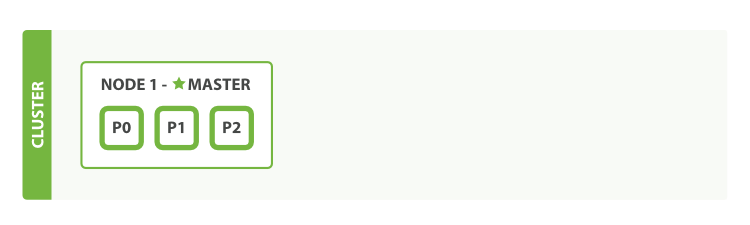
\includegraphics[width=0.6\textwidth]{elasticsearch/clustershard1.png}
\label{fig:clustershard1}
\caption{Cluster minimal, 1 node, 1 index}
\end{figure}

La santé de notre serveur est ici considéré comme moyenne, il peut parfaitement 
fonctionner, mais touts ses shards répliqués ne sont pas  actifs. En faite aucun 
shard répliqué n'est actif. Cela n'aurait pas d'intérêt d'ajouter les shards répliqués
sur ce node, car cela n'améliorera pas le traitement des données et ne protégera pas
notre cluster contre la perte de données, en cas défaillance de son unique node.

Nous allons maintenant rajouté un node, sans changer notre configuration.

\begin{figure}[H]
\center
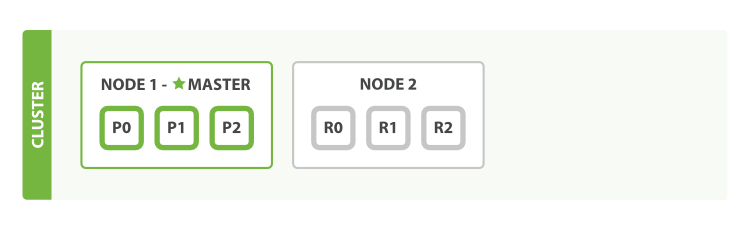
\includegraphics[width=0.6\textwidth]{elasticsearch/clustershard2.png}
\label{fig:clustershard2}
\caption{Cluster, 2 node, 1 index}
\end{figure}

On constate que notre cluster est maintenant redondé, le node master possède les 
shards primaires, le second node les shards répliqués. Ces actions sont effectuées
automatiquement à l'ajout du node.\\[2mm]

Pour plus d'informations sur la \textbf{gestion de cluster}, se référer p\pageref{subsec:elasticcluster}\\[2mm]


Cette partie permet de résoudre les problèmes qui pourraient survenir (meme sur
un cluster d'une seule machine) et permet surtout de mieux comprendre le fonctionnement
interne de Elasticsearch.

\subsection{Le tuning}
\label{subsec:elastictuning}
Voici quelques conseils applicables dans pratiquement toutes les situations et 
permettant d'optimiser le fonctionnement d'Elasticsearch.

\subsubsection{Ne pas utiliser la swap}
Il est très fréquent (et souvent nécessaire) de formater une partition de swap pour
que le système puisse optimiser son fonctionnement. C'est très pratique pour ne pas
saturer la mémoire RAM de nos machines de bureau, notamment quand on voit la consommation
pantagruélique de certains navigateurs internet récents. Les fichiers qui ne sont 
susceptibles de ne pas être utilisés avant un long moment sont parfois stockés sur le
disque dur afin de libérer de l'espace pour d'autres applications, la swap est
également utilisé lorsque l'on met un ordinateur en veille \ldots

La situation n'est pas la même sur un serveur. Ici nous sommes relativement maitre
de notre environnement et nous voulons que le service Elasticsearch soit 
le plus véloce possible. Pour se faire il faut au contraire l'empêcher au maximum 
d'utiliser la partition de swap (forcément plus lente que la RAM).

Il existe plusieurs façon de faire (y compris ne pas utiliser de partition de swap).
Celle que j'ai choisie d'utiliser est de modifier la variable \ipath{vm.swapiness}
dans le fichier \ipath{/etc/sysctl.conf}. La swapiness représente le pourcentage
de mémoire RAM restant à partir duquel on commence à envoyer de informations en
swap.

\begin{lstlisting}[style=code,label={lst:configswapiness},caption={Configuration swapiness}]
vm.swapiness = 2
swapoff -a
swapon -a
\end{lstlisting}
Il existe deux méthodes pour que le changement de swapiness soit pris en compte :
redémarrer la machine ou bien désactiver puis réactiver la swap, via les commandes
swapon, swapoff. Utiliser la commande swapoff est également une mesure radicale à 
notre problème.

\subsubsection{Utiliser une quantité de RAM raisonné}
Elasticsearch est limité par Java. Avant de parler de ces limites, il faut rappeler 
que Elasticsearch est un front-end à Apache Lucene. Lucene est conçu pour tirer 
parti très efficacement du cache des système de fichiers (probablement ext4 si 
vous utilisez Debian), qui sont en définitif, gérer par le 
noyau\footnote{https://www.elastic.co/guide/en/elasticsearch/guide/current/\_limiting\_memory\_usage.html}.
Il est conseillé par la documentation de donner au maximum 50\% de la mémoire RAM
disponible à Elasticsearch, le reste étant dédié à lucène et au bon fonctionnement
du système.
%Dans notre installation dont nous parlerons plus en détail ultérieurement, nous 
%avons choisi de nous réserver une bonne marge de manœuvre puisqu'un redis et un Logstash
%minimalistes tournent en sus sur la machine hébergeant Elasticsearch.

Cependant cette valeur de 50\% n'a de sens que si Elasticsearch consomme moins de 
32Go de RAM. En allouer plus devient contreproductif. Jusqu'à 32Go
la machine virtuelle Java (JVM) \textit{compresse} les adresses des pointeurs 
(tant qu'on reste sous la limite des 32Go de RAM on peut continuer à utiliser les 
adresses mémoires sur 4 octets), après, la consommation de mémoire explose et le
\textit{garbage collector} devient bien moins efficace.

Pour les machines possédant une énorme quantité de mémoire RAM (128Go à 1To)
il conseiller pour optimiser le fonctionnement de la machine de faire tourner plusieurs
noeuds d'Elasticsearch dessus (attention aux entrées sortie et à l'utilisation processeur).

\subsection{Faire du nettoyage régulièrement}
Plus Elasticsearch agrège des données plus il s'empâte, ce phénomène est inévitable 
sur le long terme. Les contre-mesures sont de scale-out (monter à l'échelle horizontalement)
en rajoutant de nouveaux nœuds au cluster. 

Pour éviter ce ralentissement la solution la plus radicale reste de supprimer les 
données. Justement, dans le cadre de notre projet, nous n'avons pas besoin de conserver 
toutes les données sur le long terme. Nous avons donc décider de supprimer les logs 
de changement d'état des par-feu tous les 4 jours. Ces logs peuvent représenter 
jusqu'à 30Go de données journalières. 
Pour ce faire nous utiliserons un tâche \textbf{cron} couplé à un script bash 
\ref{lst:scriptdelindex} tirant parti de l'API d'Elasticsearch dont nous parlerons 
plus bas. Pour indication, les index de firewall son supprimés tous les 4 jours, 
(une requête judiciaire/alerte sécurité arrive en général en moins de 3 jours).\\ 
Les logs sont de toute façon également conservés ailleurs pour se soumettre aux 
imperatifs judiciaires. Les index d'état (intéressants pour établir des statistiques)
sont conservés 1 mois.\\[2mm]
Zoom sur la commande curl et son utilisation dans cron

\begin{lstlisting}[style=code,label={lst:curlexemple},caption={Extrait de notre script \ref{lst:scriptdelindex}}]
curl -sS -XDELETE $blade:$port/$target-$d
\end{lstlisting}

On remarque ici l'utilisation de l'option -sS pour \textit{silent, Show errors}.
Ainsi cron n'est pas importuné par les retour sur la sortie standard cela permet
également, en ajoutant la directive \textbf{MAILTO: mail@example.fr} de renvoyer
la sortie d'erreur vers mail@example.fr. Cela nécessite évidemment d'avoir configurer
un serveur mail sur notre machine, par défaut sur Debian, Exim (dpkg-reconfigure 
exim-config).

Concernant -XDELETE c'est une utilisation de l'API REST décrite plus bas.

Une des stratégies préconisé dans le cas où l'on souhaite conserver des données sur
le long terme alors qu'on en a seulement un besoin d'accès et d'analyse ponctuel ;
consiste à les enregistrer dans des fichiers séparés (output Logstash) et de les 
faire ingérer à un cluster Elasticsearch dimesinonné en conséquence le moment venu.


\section{Les API Elasticsearch}
Elasticsearch est énorme, mais peut être assez facilement utilisable par le 
plus grand nombre grâce aux \gls{API} \emph{optimisées} pour chaque tâches qui ont été implémentées.\\[2mm]
Pour faciliter l'utilisation des différentes APIs il est conseillé d'utiliser \textbf{Sense},
cet outil est présenté p\pageref{subsec:elasticsense}


\subsection{API REST}
Cette API sert à la communication avec Elastisearch, comme toutes les API REST elle
utilise les méthodes HTTP, ici : GET, POST, PUT et DELETE et s'appuie ensuite sur l'architecture d'Elasticsearch.

\textbf{{\color{grey}http://host:port}/[{\color{red}index}]/[{\color{cyan}type}]/[{\color{yellow}\_action/id}]}\\[4mm]
Imaginons que dans un projet fictif, nous souhaitions référencer des tweets.
On pourrait procéder comme suit pour ajouter le premier.

\textbf{PUT  {\color{grey} http://100.127.255.1:9200}/{\color{red}twitter}/{\color{cyan}tweet}/{\color{yellow}1}}

\begin{lstlisting}[style=code,label={lst:RESTexemple1curl},caption={Avec curl}]
curl -XPUT http://100.127.255.1:9200/twitter/tweet/1
\end{lstlisting}
%Voici le résultat en utilisant curl, directement en ligne de commande, par 
%navigateur, \ldots

\begin{lstlisting}[style=code,label={lst:RESTexemple1sense},caption={Avec Sense}]
PUT /twitter/tweet/1
\end{lstlisting}

Voici la syntaxe que nous obtiendrions en utilisant Sense, puisque notre serveur 
et notre port sont déjà renseignés. Nous utiliserons par convention cette syntaxe plus courte.

La directive \textbf{PUT} est utilisé pour renseigner de nouvelles informations dans Elasticsearch.\\[2mm]
Dans notre projet d'analyse de logs, il est fréquent que nous dussions supprimer 
des index, notamment dans le cas du paramétrage des \emph{mappings}, mais également
pour soulager notre infrastructure du poids des logs de firewall (~20-30Go/jours).\\

\textbf{DELETE  {\color{grey} http://100.127.255.1:9200}/{\color{red}twitter}/}\\

Si nous avions un index twitter journalier il serait possible d'utiliser une commande
très similaire pour supprimer tous les index d'un seul coup :\\

\textbf{DELETE  {\color{grey} http://100.127.255.1:9200}/{\color{red}twitter*}}\\

La directive \textbf{DELETE} est utilisé pour supprimer des informations d'Elasticsearch.\\


La directive \textbf{GET} sert à récupérer des information à tout niveaux: index,
type, mapping\ldots Il faut par contre avoir l'identifiant exact de la ressource à laquelle on souhaite accéder pour utiliser cette directive.
Ce n'est pas un outils de recherche\footnote{Outils de recherche abordé dans la section suivante}.\\[2mm]
\textbf{GET  {\color{grey} http://100.127.255.1:9200}/{\color{red}twitter}/{\color{cyan}tweet}/{\color{yellow}1}}\\

Les réponses d'Elasticsearch sont en \textbf{JSON}. 


\subsection{Les API de recherche}
%DSL pour Domain Specific Language, parce que Elasticsearch est avant tout un moteur 
%de recherche, il dispose de puissantes fonctionnalités de recherche. Il dispose donc
%de son propre langage d'interrogation le QueryDSL. C'est loin d'être un cas unique,
%par exemple Puppet dispose également de son propre langage de configuration.

Il existe plusieurs API (ou méthodes) de recherche dans Elasticsearch nous les  
détaillerons plus en détail l'API searchLite après avoir expliqué le fonctionnement général d'une recherche dans Elasticsearch.

La recherche dans Elasticsearch est particulièrement efficace, car Elasticsearch 
indexe tout le contenu de ses documents (il indexe chaque champ, en fonction d'un
mapping particulier\footnote{explication sur le mapping p\pageref{sec:mappingetanalys}}).
%C'est pour faciliter l'indexation qu'Elasticsearch utilise du JSON structuré.

\subsubsection{Empty Search}
C'est la forme la plus basique de l'API de recherche, on ne spécifie pas de requête
spécifique. Comprendre le fonctionnement et les possiblité de cette API basique 
permettra d'utiliser plus efficacement SearchLite, qui en est l'évolution directe.


\begin{lstlisting}[style=code,label={lst:APIsearchemptyexample1},caption={le "Hello World" de la recherche}]
GET /_search
\end{lstlisting}

Cette requête retourne tous les documents, de tous les index du cluster duquel nous
sommes membre.

\begin{lstlisting}[style=code,label={lst:APIsearchemptyexample2},caption={Réponse type à notre requête précédente}]
{
    "took": 798,
    "timed_out": false,
    "_shards": {
        "total": 201,
        "successful": 201,
        "failed": 0
    },
    "hits": {
        "total": 353585048,
        "max_score": 1,
        "hits": [
        {
            "_index": ".kibana",
            "_type": "visualization",
            "_id": "Top5-nat-firewall-router",
            "_score": 1,
            "_source": {
                "title": "Top5 nat-firewall router",
                "visState": "{\"type\":\"histogram\",\"params\":{\"shareYAxis\":true,\"addTooltip\":true,\"addLegend\":true,\"mode\":\"stacked\",\"defaultYExtents\":false},\"aggs\":[{\"id\":\"1\",\"type\":\"count\",\"schema\":\"metric\",\"params\":{}},{\"id\":\"2\",\"type\":\"terms\",\"schema\":\"group\",\"params\":{\"field\":\"IPnat\",\"size\":5,\"order\":\"desc\",\"orderBy\":\"1\"}}],\"listeners\":{}}",
                "description": "",
                "version": 1,
                "kibanaSavedObjectMeta": {
                "searchSourceJSON": "{\"index\":\"firewall-*\",\"query\":{\"query_string\":{\"query\":\"*\",\"analyze_wildcard\":true}},\"filter\":[]}"
                }
            }
        },
        .... 9 Autres ...
    }
}
\end{lstlisting}

Quelques explications :

\paragraph{hits}
L'élément hits contient des informations sur la requête et les réponse à la requête.
\textit{total} représente le nombre total de documents retournés pour cette requête, ici le 
nombre total de documents indexés: 353585048. 
Cela signifie qu'il y avait environ 353 millions de lignes
de logs indexés dans notre Elasticsearch au moment de la requête.

Les réponses à la requête nous sont renvoyées dans l'array \textit{hits}, par défaut
seul les 10 premiers documents satisfaisant notre requête nous sont renvoyés 
(comme il n'y avait pas de requête, simplement les 10 premiers documents).

Les documents renvoyés dans l'array sont classés en fonction de leur \_score, une 
fois encore, puisque nous n'avons rien précisé dans notre requête, tous les résultats 
nous sont renvoyés avec le score 1.

On notera que le \ipath{max\_score}, score maximum obtenu lors de la requête.

Enfin on remarque que le source (tous les champs indexés) de chaque document est présent
dans la réponse à la requête.

\paragraph{took}
Took est le temps en millisecondes pris pour effectué cette requête, ici 798ms

\paragraph{shard}
L'élément \_shards, nous indique le nombre de shards utilisé lors de la requête. 
Dans combien de shards tout c'est bien passé, dans combien il y a eu des erreurs.
Les erreurs sont très peu probables, cela se produit généralement sur un cluster 
de plusieurs machines, alors que plusieurs d'entre elles sont inacessibles (il faut 
que les primary et replica d'un shard soient inaccessible en même temps). Cela peut aussi produire sur un serveur surchargé (les temps d'accèstrop long feront croire à Elasticsearch que le shard est inaccessible).

\paragraph{timeout}
Il est possible d'effectuer une recherche \textit{par timeout}, cela signifie que 
Elasticsearch va effectuer sa recherche de façon classique, mais que lorsque le temps
autorisé pour la recherche est dépassé, il renvera les informations 
qu'il a eu le temps de rassembler. Toujours dans l'ordre qui lui semble le plus pertinant
(ordonné par score). Attention cependant, cela ne nous absouds pas pour autant du
coût de la recherche. Si les shards renvoient bien les résultats pertinents au moment
souhaité, cela n'arrête pas pour autant la requête qui finira de s'executer en arrière
plan même si les résultats ne sont pas pris en compte.

\begin{lstlisting}[style=code,label={lst:APIsearchemptyexample3},caption={Une recherche "vide" avec timeout}]
GET /_search?timeout=10ms
\end{lstlisting}


\paragraph{Recherche multi-index et multitype}
La recherche multi-index et multitype est toujours possible comme dans l'API REST

\begin{lstlisting}[style=code,label={lst:APIsearchemptyexample4},caption={Une recherche multi-index ...}]
GET /gb,us/_search
GET /g*,u*/_search
GET /gb,us/user,tweet/_search
\end{lstlisting}

\paragraph{Pagination}
Par défaut lors d'une requête Elasticsearch renvoit seulement les 10$^{ers}$ résultats.
Il est biensure possible de paramétrer cela, pour afficher plus de résultats, et pas
forcément les plus pertinents (ceux qui présente le score le plus élevé).\\
\textbf{size} permet d'indiquer le nombre de résultats souhaités\\
\textbf{from} permet d'indiquer le nombre de résultats que l'on souhaite sauter.

\begin{lstlisting}[style=code,label={lst:APIsearchemptyexample4},caption={Pagination}]
GET /_search?size=5&from=10
\end{lstlisting}

Maintenant que nous savons utiliser les requêtes dans Sense, voilà celle que l'on
utilise pour connaitre la santé de son cluster (notion abordé p\pageref{subsec:labase})

\begin{lstlisting}[style=code,label={lst:elastichealth},caption={Santé du cluster}]
GET /_cluster/health
\end{lstlisting}


\subsubsection{Search Lite}
\label{subsec:elasticsearchlite}
Comme expliqué avant il existe deux formes d'API de recherche. L'API lite avec requête
en chaine de caractères \textit{(string query)} et l'API \textit{"full body request"},
qui nécessite comme corps de la requête, du JSON\footnote{Voir la documentation}.

Utiliser la recherche SearchLite, nécessite simple d'ajouter à notre
empty search \emph{?q=} puis la requête. 
\emph{Attention, si vous utilisez cette API avec 
curl, \emph{il pourrait être nécessaire d'utiliser la syntaxe http} (\%2B pour + par exemple)}.

\begin{lstlisting}[style=code,label={lst:APIsearchliteexample1},caption={Exemples simples}]
GET /_search?q=epinal
GET /state-2015.05.22/_search?q=epinal
\end{lstlisting}

Ici on cherche le terme \emph{epinal} dans tous les champs, c'est par fois utile,
mais dans de nombreux cas nous connaissons déjà le nom du champ (cf \hyperref[lst:grokregex1]{Logstash}) dans
lequel nous souhaitons avoir le terme. 

Pour se faire il suffit d'utiliser la syntaxe suivante : 
\begin{lstlisting}[style=code,label={lst:APIsearchliteexample2},caption={Choix du champ}]
GET /_search?q=logsource:epinal
\end{lstlisting}

Bien plus intéressant, il est possible d'imposer des conditions à remplir ie: doit
contenir le terme suivant, ou au contraire ne doit \textbf{pas} contenir le terme 
suivant.

\begin{lstlisting}[style=code,label={lst:APIsearchliteexample3},caption={Conditions must (not) match}]
GET /_search?q=+logsource:*epinal* -logsource:sw*
\end{lstlisting}

Dans l'exemple précédant on souhaite chercher les équipement réseaux situés à epinal
mais pas les switchs.
L'utilisation des + et - change vraiment le sens de la requête, dans la précédante
sans les symboles, la présence ou non augmentait la pertinence des réponses contenant
le terme recherché, mais n'était pas discriminante.
Avec ces symboles, on exclu les réponses qui ne se conforment pas à nos exigences.


La présence des \textbf{*} est une sorte de globbing, nécessaire lorsque l'on fait
une recherche fulltext 


Il existe un autre moyen d'influencer la pertinence des résultats (de faire remonter
en haut de liste ce qui nous intéresse le plus).
Cela est particulièrement pratique dans les longues requêtes.
Il s'agit de l'opérateur \textbf{\^} qu'on n'utilise en général en conjonction de
parenthèses (qui servent simplement à faire des groupes).


\begin{lstlisting}[style=code,label={lst:APIsearchliteexample4},caption={Modifier la pertinence}]
GET /_search?q=+logsource:*epinal* -logsource:sw* (timestamp:May)^10 Power
\end{lstlisting}
Dans cette requête nous cherchons toujours des équipements non switch situés à Epinal.
Nous somme cette fois ci très intéressés par ce qui s'est passé en Mai et d'autant
plus si cela concerne un problème d'alimentation éléctrique.

Concernant la gestion du temps, et des timestamp, nous allons voir une propriété 
intéressante d'Elasticsearch lorsque le mapping de l'index est bien réalisé.
Il est capable de \textit{s'orienter} dans le temps à partir d'un champ texte.
Cela n'est pas forcément très utile si l'on utilise Kibana, puisque son interface
nous permet très facilement d'être plus précis, mais cela laisse imaginer les possiblités
d'Elasticsearch.


\begin{lstlisting}[style=code,label={lst:APIsearchliteexample5},caption={Le temps dans SearchLite}]
GET /_search?q=+logsource:*epinal* -logsource:sw* (timestamp:>Jun)^10 Power
GET /_search?q=+logsource:*epinal* -logsource:sw* (timestamp:=<Jun)^10 Power
\end{lstlisting}

SearchLite accepte les opérateur $< > =< =>$ et Elasticsearch est capable de les 
interpréter pour peu que le champ soit \textit{mappé comme date}(cf Mapping).

Il est possible d'utiliser les opérateurs logiques \textbf{OR} et \textbf{AND} 
dont l'utilisation est assez évidante \ldots
\begin{lstlisting}[style=code,label={lst:APIsearchliteexample6},caption={Opérateurs logiques}]
+IPoutside:"8.8.8.8" +IPnat:"8.8.4.4" +(portnat:"37657" OR portnat:"19474")
\end{lstlisting}

Il faut faire attention à l'utilisation des symboles -, :, /," qui on une signification.


Remarque générale, les syntaxes présentées jusqu'à présent son utilisables telles
quelles dans Sense, et en retirant \ipath{GET /\_search?q=} dans Kibana.


%\subsubsection{Full-Body Search et QueryDSL}
%{\huge TODO!}

\section{Le mapping et l'analyse}
\label{sec:mappingetanalys}
\subsection{Mapping}
Le mapping est \textbf{comparable au schéma d'une base, dans le modèle relationnel}.
Le mapping définit donc le "type" de nos "champs". Attention on fait rentrer dans 
le mapping plus, que dans le schéma d'une base (analyse, indexation, \ldots).

Il y'a un mapping différent par index (il existe aussi des templates, applicable 
à plusieurs index). Pour accéder au mapping d'un index il suffit dans Sense de lancer
la requête suivante.

\begin{lstlisting}[style=code,label={lst:mappingget1},caption={Obtenir un mapping}]
GET /firewall-2015.05.07/_mapping
\end{lstlisting}

Voir un \textbf{exemple de mapping} : p\pageref{lst:mappingresult}\\[2mm]



On remarque que beaucoup de champs ont pour type \textbf{string}, c'est le type choisi
par défaut.

Bien qu'ils ne soient pas utilisés ici il existe d'autres types de base, il est aussi
possible d'en définir soi-même, cela ne sera pas abordé dans ce rapport.

Types par défaut :
\begin{itemize}
    \item   boolean: true/false
    \item   long: nombres entiers
    \item   double: nombres à virgule
    \item   string: chaine de charactères
    \item   date:   une date valide, (voir la doc pour les normes acceptées)
\end{itemize}

Pour créer un nouveau mapping, il faut au préalable supprimer le précédent, (supprimer 
l'index auquel est attaché le mapping).


\begin{lstlisting}[style=code,label={lst:mappingiput1},caption={Changer le mapping d'un index}]
DELETE /firewall-2015.05.07
PUT /firewall-2015.05.07/
{
    "mappings": {
    ....
             "properties": {
                "@timestamp": {
                "type": "date",
                "format": "dateOptionalTime"
                },
                "@version": {
                "type": "string",
                "index": "not_analyzed"
                },
                "IPinside": {
                "type": "ip",
                "index": "analyzed",
                "store": "yes"
                },
                "IPnat": {
                "type": "string",
                "index": "not_analyzed",
                "norms": {
                "enabled": false
                },
                }
                ....
            }
    }
}
\end{lstlisting}

La requête entière est trop longue pour être affiché, donne une idée de la forme.
Une méthode efficace pour générer la sienne est d'utiliser le mapping créé par Elasticsearch
par défaut puis modeler notre requête à notre convenance à partir de ce squelette.

Cette méthode est pratique pour faire des tests mais elle ne concerne qu'un seul 
index. Dans le projet nous travaillons avec de multiples index, il sera plus pratique
d'utiliser les templates pour que le même modèle s'applique partout où nous le souhaitons.

Autre remarque, \textbf{si vous faites la manipulation ci-dessus dans un environnement de 
production, il y a toutes les chanches pour qu'Elasticsearch vous renvoie une erreur}.
Par défaut Logstash créé de nouveaux index si rien n'existe pour accueillir les logs qu'il envoie à Elasticsearch. Ainsi, si on supprime l'index du jour (on perd les données), mais un autre index du même nom sera recréer avecle template par défaut presque 
instantanément puisque Logstash reçoit (dans notre cas) environ \textbf{500logs/s}. 
Pendant les tests il peut être judicieu d'éteindre Logstash.


Un template sera ici le mapping par défaut utilisé par une certaine forme d'index, une sorte de modèle.
Pour créer un template, il faut simplement supprimer l'ancien et écrire le nouveau.
Il est également conseillé de supprimer les anciens index utilisant un mapping 
différent. Ils seront \textbf{toujours utilisables dans Sense}, mais seront 
\textbf{incohérents aux yeux de Kibana} et empêcheront de faire des recherches
\footnote{Faire des recherches avec des mappings différents, c'est comme faire des opérations dans des bases différentes}.\\[2mm]


Voir un exemple de \textbf{création de template} p\pageref{lst:mappingput2}\\[2mm]

%On constate que certains champs sont analysés et d'autres non, ces choix apparaitrons
%plus clairs après la partie concernant l'analyse.
Du point de vue mapping on peut noter que integer est également un type valable (liste 
exhaustive dans la documentation), on constate aussi que le type date (un type particulier
de string), qui \textbf{ne peut pas} être analysé, supporte plusieurs formats, définis
d'après la \hyperref[http://joda-time.sourceforge.net/api-release/org/joda/time/format/DateTimeFormat.html]{norme JAVA}\footnote{http://joda-time.sourceforge.net/api-release/org/joda/time/format/DateTimeFormat.html}.
Avec quelques types prédéfinis \hyperref[https://www.elastic.co/guide/en/elasticsearch/reference/1.5/mapping-date-format.html]{ici}\footnote{https://www.elastic.co/guide/en/elasticsearch/reference/1.5/mapping-date-format.html}.


\subsection{Analyse}
On remarque que certains champs ont également un \textbf{index: "not\_analyzed"}.
Tous n'en n'ont pas car il est souvent plus intéressant d'avoir des champs analysés.
Et par défaut tous les champs sont analysés.

Il existe trois niveaux d'indexation:
\begin{itemize}
    \item   \textbf{Analyzed}, signifie que la chaine de caractère est analysé puis indexé,
    donc cherchable en \textit{full text}.
    \item   \textbf{not\_analyzed}, le champ est toujours cherchable, mais puisqu'il n'a pas 
    été analysé, on ne peut le trouvé qu'avec sa valeur exact. \emph{Cette propriété
    peut se révéler essentielle pour réaliser des graphiques efficaces.} 
    \footnotesize{Il faut parfois savoir comment on veut exploiter ses données pour
    pouvoir les traiter en conséquence.}
    \item \textbf{no}, n'index pas ce champ, il n'est pas cherchable. Je ne me suis
    jamais servis de cette propriété, peut sans doute avoir une utilité pour l'optimisation
    de performances.
\end{itemize}

\subsubsection{Fonctionnement de l'analyse}
L'analyse consiste en deux grandes étapes, découper une chaine de charactère en termes
recherchable, puis assainissement de ces termes en enlevant par exemple les majuscules
ou en retirant les termes non pertinents (le, la, les, des \ldots), voir même en 
remplaçant des synonymes.

En fait le processus compte trois étapes. Tout d'abord le \emph{filtrage de caractères}
(faire disparaitre les / ou transformer \& en et. La tokenization (\textit{termisation}
en traduction approximative), créer un terme pour chaque chaine de caractère séparer
par un espace, une virgule, un point, \ldots{} (paramétrable cf doc). Enfin le filtre
de termes, (décris dans l'assainissement au dessus).\\[2mm]

Le fonctionnement des \textbf{recherches full text} est expliqué plus en détail p\pageref{subsec:elasticfulltext}


\section{Conclusion}
Nous savons maintenant ranger nos données de façon efficace dans Elasticsearch cela va nous permettre de créer des index faciles à analyser et à \textit{requêter} avec Kibana. Cette partie est probablement la pluscomplexe et la plus importante mais aussi la moins user-friendly. 
Construire un mapping n'est pas facile et nécessite de bien comprendre anticiper l'exploitation que l'on souhaite faire de ses données.



%\section{Plus d'information }
